% ============================================================
%  Delta-Neutral ETH Carry Strategy — Final Report
%  Compile with: pdflatex final_report.tex
% ============================================================
\documentclass[11pt,a4paper]{article}

% --- Encoding & font ---
\usepackage[T1]{fontenc}
\usepackage[utf8]{inputenc}
\usepackage{lmodern}

% --- Page geometry ---
\usepackage[top=1in, bottom=1in, left=1in, right=1in]{geometry}

% --- Math ---
\usepackage{amsmath}
\usepackage{amssymb}

% --- Tables ---
\usepackage{booktabs}
\usepackage{array}

% --- Code listings ---
\usepackage{listings}
\usepackage{xcolor}

% --- Graphics ---
\usepackage{graphicx}
\graphicspath{{../output/charts/}}
\usepackage{caption}
\usepackage{subcaption}

% --- Hyperlinks ---
\usepackage{hyperref}
\hypersetup{
    colorlinks=true,
    linkcolor=black,
    urlcolor=blue,
    citecolor=black,
    pdfauthor={},
    pdftitle={Delta-Neutral ETH Carry Strategy}
}

% --- Headers / footers ---
\usepackage{fancyhdr}
\pagestyle{fancy}
\fancyhf{}
\lhead{\small Delta-Neutral ETH Carry Strategy: On-Chain Proof-of-Concept and Backtest}
\rhead{\small\thepage}
\renewcommand{\headrulewidth}{0.4pt}

% --- Section formatting ---
\usepackage{titlesec}
\titleformat{\section}{\large\bfseries}{\thesection.}{0.5em}{}
\titleformat{\subsection}{\normalsize\bfseries}{\thesubsection}{0.5em}{}
\titleformat{\subsubsection}{\normalsize\itshape}{\thesubsubsection}{0.5em}{}

% --- Paragraph spacing ---
\usepackage{parskip}
\setlength{\parskip}{6pt}
\setlength{\parindent}{0pt}

% --- Lists ---
\usepackage{enumitem}
\setlist{noitemsep, topsep=4pt}

% --- Listings style ---
\definecolor{codebg}{rgb}{0.95,0.95,0.95}
\definecolor{codeframe}{rgb}{0.75,0.75,0.75}
\definecolor{commentcolor}{rgb}{0.4,0.4,0.4}
\definecolor{keywordcolor}{rgb}{0.1,0.1,0.6}
\definecolor{stringcolor}{rgb}{0.2,0.5,0.2}

\lstset{
    backgroundcolor=\color{codebg},
    frame=single,
    rulecolor=\color{codeframe},
    basicstyle=\ttfamily\small,
    keywordstyle=\color{keywordcolor}\bfseries,
    commentstyle=\color{commentcolor}\itshape,
    stringstyle=\color{stringcolor},
    breaklines=true,
    breakatwhitespace=true,
    numbers=none,
    xleftmargin=6pt,
    xrightmargin=6pt,
    aboveskip=8pt,
    belowskip=8pt,
    showstringspaces=false,
    tabsize=4,
}

\lstdefinestyle{solidity}{
    language=C,
    morekeywords={function,public,external,internal,pure,view,returns,
                  require,mapping,address,uint256,uint128,uint8,int256,
                  bool,bytes32,string,emit,event,modifier,struct,interface,
                  library,contract,is,new,delete,memory,storage,calldata,
                  immutable,override,virtual,constructor,onlyOwner,nonReentrant},
}

\lstdefinestyle{javascript}{
    language=C,
    morekeywords={const,let,var,async,await,import,from,export,default,
                  function,return,true,false,null,undefined,new,this},
}

% ============================================================
\begin{document}
% ============================================================

% --- Title block ---
\begin{center}
    {\LARGE\bfseries Delta-Neutral ETH Carry Strategy:\\[4pt]
    On-Chain Proof-of-Concept and Backtest}\\[12pt]
    {\normalsize
        \textbf{Course:} [Course Name] \quad
        \textbf{Team:} [Names]\\[4pt]
        \textbf{Date:} [Date] \quad
        \textbf{Testnet:} Sepolia \quad
        \textbf{Repository:} [GitHub URL]
    }
\end{center}
\hrule
\vspace{10pt}

% ============================================================
\section*{Abstract}
% ============================================================

This project designs, implements, and analyses a delta-neutral ETH carry strategy that simultaneously holds a long ETH spot allocation and a short ETH perpetual futures position of equal notional. The two legs approximately cancel price risk, leaving the perpetual funding rate as the net income source. We built five verified Solidity smart contracts on the Sepolia testnet --- including a Chainlink oracle integration and a rule-based strategy vault --- as an on-chain proof-of-concept of the mechanism. A backtest using Bybit ETHUSDT 1-hour data (Jan 2021 -- Mar 2026, $\approx$45,900 hourly bars) measures historical profitability across a full market cycle with a carry entry gate, decomposing returns into funding carry, transaction costs, and hedge residual. With the carry gate active, the strategy generated \textbf{+\$18,442 net profit (+35.2\% annualised)} on \$10,000 capital over the 5-year window, sitting out approximately 21\% of the period during backwardation regimes. The Sharpe ratio is heavily influenced by elevated funding rates during the 2021 bull market; the post-2021 figure is approximately 0.4.

\hrule\vspace{6pt}

% ============================================================
\section{Introduction}
% ============================================================

\subsection{Motivation}

Perpetual futures markets in crypto operate through a funding rate mechanism: when long demand exceeds short demand, the contract price rises above spot, and a periodic payment transfers from long traders to short traders to enforce price convergence. In crypto bull markets, retail investors exhibit a systematic long bias --- they want leveraged upside exposure to assets like ETH. This creates persistent positive funding rates (contango), which short sellers systematically collect as income. By combining a long spot position with a short perpetual of equal notional, a trader can harvest this funding premium with approximately zero net price risk. This is the \emph{delta-neutral carry trade}.

\subsection{Project Objective}

This project has two objectives:

\begin{enumerate}
    \item \textbf{Academic:} Analyse the historical profitability of a delta-neutral ETH carry strategy using Bybit ETHUSDT historical data. Measure how the strategy performs across different funding rate regimes, and whether funding income meaningfully exceeds the benchmark opportunity cost after costs.

    \item \textbf{Implementation:} Deploy a working on-chain proof-of-concept on Sepolia that correctly implements the vault structure, carry entry gate, exit conditions, and PnL accounting --- demonstrating that the mechanism can be enforced in Solidity.
\end{enumerate}

\subsection{Scope and Limitations}

\begin{itemize}
    \item \textbf{Not a live trading system.} No real exchange connectivity. \texttt{MockPerpEngine} simulates perpetual mechanics without order books, counterparties, or real settlement.
    \item \textbf{Backtest uses a local CSV file.} Data is sourced from Bybit (\texttt{data/raw/bybit\_eth\_usdt\_1h.csv}). The backtest does not pull live feeds.
    \item \textbf{No rebalancing.} The basic backtest holds a fixed 1:1 notional position throughout with no delta rebalancing.
    \item \textbf{On-chain and backtest layers are independent.} The contracts do not execute the historical backtest; they demonstrate the mechanism.
\end{itemize}

\subsection{Report Structure}

Section~2 covers background on perpetual futures and funding rates. Section~3 defines the strategy. Section~4 presents the mathematical model. Section~5 covers the smart contract design. Section~6 covers oracle design. Section~7 covers deployment. Section~8 presents backtest results. Section~9 describes the frontend. Section~10 covers gas analysis. Section~11 discusses risks. Section~12 concludes.

% ============================================================
\section{Background}
% ============================================================

\subsection{Perpetual Futures and Funding Rates}

A perpetual futures contract tracks an underlying asset without an expiry date. Without expiry, a separate mechanism is needed to keep the contract price anchored to spot. Exchanges use a \textbf{funding rate}: at regular intervals (every 8 hours on major exchanges), a payment is transferred between long and short position holders proportional to the divergence between mark price and index price:

\[
    \text{fundingRate} = \frac{\text{markPrice} - \text{indexPrice}}{\text{indexPrice}}
\]

When the funding rate is positive (mark above spot, contango), long traders pay short traders. When negative (backwardation), short traders pay long traders. This mechanism prevents the perpetual from drifting permanently from the underlying.

\subsection{Why Contango Persists in Crypto}

Crypto retail investors exhibit a strong long bias --- they seek leveraged upside exposure to ETH and BTC. Perpetual futures are the primary vehicle. This excess long demand persistently pushes the mark price above spot in bull and neutral markets, generating a positive funding rate. Historical data shows that the average ETH perpetual funding rate has been positive over most of the 2021--2024 period, ranging from approximately 0.01\% per 8-hour period in quiet markets to over 0.1\% during peak bull markets. Short sellers who hold positions through these periods collect this income systematically.

\subsection{The Delta-Neutral Cash-and-Carry}

A pure cash-and-carry trade holds a spot ETH long and an equal short perp. Price moves cancel:
\begin{itemize}
    \item ETH rises by $X$\%: spot position gains $X$\%, perp short loses $X$\% $\Rightarrow$ net price PnL $= 0$
    \item ETH falls by $X$\%: spot position loses $X$\%, perp short gains $X$\% $\Rightarrow$ net price PnL $= 0$
\end{itemize}

The only net income is the funding rate received on the short leg, minus the opportunity cost of the capital. This is analogous to a basis trade in traditional finance.

% ============================================================
\section{Strategy Definition}
% ============================================================

\subsection{Position Structure}

\begin{table}[h!]
\centering
\caption{Position structure of the delta-neutral carry strategy.}
\begin{tabular}{@{}llll@{}}
\toprule
\textbf{Component} & \textbf{Size} & \textbf{Direction} & \textbf{Purpose} \\
\midrule
Spot allocation    & $=$ Capital         & Long  & Tracks ETH price, cancels perp price risk \\
Perp notional      & $=$ Capital         & Short & Collects funding income in contango \\
Perp collateral    & 20\% of notional    & Posted margin & Supports $5\times$ leverage on the short \\
\bottomrule
\end{tabular}
\end{table}

\subsection{Profit Sources}

The daily net PnL decomposes as:

\begin{align}
    \text{daily net PnL} &= \text{spot\_pnl} + \text{perp\_pnl} + \text{funding\_income} - \text{benchmark\_cost} \notag \\[4pt]
    \text{spot\_pnl}       &= \text{notional} \times \left(\frac{p_t}{p_{t-1}} - 1\right) \notag \\
    \text{perp\_pnl}       &= -\text{spot\_pnl} \quad \text{(exact mirror, cancels)} \notag \\
    \text{funding\_income} &= \text{notional} \times \text{dailyFundingRate} \notag \\
    \text{benchmark\_cost} &= \text{capital} \times \frac{\text{benchmarkRate}}{365} \notag
\end{align}

Therefore:
\[
    \text{daily net PnL} \approx \text{funding\_income} - \text{benchmark\_cost}
    \quad \text{(price legs cancel)}
\]

\subsection{Carry Score}

The carry score measures whether the funding rate justifies entering the position relative to its opportunity cost:

\[
    \text{carryScore} = \bigl(\text{dailyFundingRate} \times 365\bigr) - \text{benchmarkRate} - \text{costs}
\]

\[
    \text{Entry when: carryScore} > \text{dynamicThreshold}
    \quad \text{where} \quad
    \text{dynamicThreshold} = \text{costs} + (\text{leverage} \times \text{riskPremium})
\]

\subsection{Why This Is Not Pure Risk-Free Arbitrage}

The strategy retains several real risks:
\begin{enumerate}
    \item \textbf{Funding reversal:} If funding turns persistently negative (backwardation), the strategy loses money even with delta-neutrality.
    \item \textbf{Margin / liquidation risk:} The short perp uses $5\times$ leverage. A sharp ETH price rise can erode the collateral buffer faster than funding income accumulates.
    \item \textbf{Execution cost drag:} Entry/exit costs, fee drag, and market impact reduce net returns.
    \item \textbf{Rebalancing risk:} As prices move, the hedge ratio drifts away from 1:1, reintroducing delta.
\end{enumerate}

% ============================================================
\section{Mathematical Model}
% ============================================================

\subsection{Core Formulas}

All formulas are implemented identically in \texttt{contracts/core/ArbitrageMath.sol} and \texttt{backtest/run\_backtest.py}.

\textbf{Spot leg PnL} (long):
\[
    \text{spotPnL} = \text{spotAllocation} \times \frac{\text{currentPrice} - \text{entryPrice}}{\text{entryPrice}}
\]

\textbf{Short perp price PnL} (equals $-\text{spotPnL}$ at equal notional):
\[
    \text{shortPricePnL} = \text{notional} \times \frac{\text{entryPrice} - \text{currentPrice}}{\text{entryPrice}}
\]

\textbf{Delta neutrality:}
\[
    \text{spotPnL} + \text{shortPricePnL} = 0
\]

\textbf{Funding income} (received by short when rate $> 0$):
\[
    \text{fundingPayment} = \text{notional} \times \frac{\text{dailyFundingRate}_{\text{bps}}}{10{,}000}
\]

\textbf{Carry score} (annualised bps):
\[
    \text{carryScore} = \bigl(\text{dailyFundingRate}_{\text{bps}} \times 365\bigr)
                        - \text{benchmarkRate}_{\text{bps}}
                        - \text{cost}_{\text{bps}}
\]

\textbf{Margin ratio:}
\[
    \text{marginRatio} = \frac{\text{collateral} + \text{unrealisedPnL}}{\text{notional}} \quad [\text{in bps}]
\]

\textbf{Break-even days:}
\[
    \text{breakEvenDays} = \frac{\text{entryCostUSDC}}{\text{dailyNetYieldUSDC}}
\]

\subsection{Backtest Formulas (from \texttt{docs/formulas.md})}

\textbf{Spot PnL per bar:}
\[
    \text{spot\_pnl} = \text{pos} \times (S_t - S_{t-1})
\]

\textbf{Perp PnL per bar:}
\[
    \text{perp\_pnl} = -\text{pos} \times (F_t - F_{t-1})
\]

\textbf{Funding PnL per bar:}
\[
    \text{funding\_pnl} = \text{pos} \times F_t \times r_{t-1}
\]
where $r_{t-1}$ is the Bybit 8h settlement rate divided by 8 (per-hour accrual).

\textbf{Basis:}
\[
    \text{basis\_pct} = \frac{F_t - S_t}{S_t} \times 100
\]

\textbf{Carry gate signal:}
\[
    \text{annFunding}_{\text{bps}} = \overline{r}^{7\text{d}} \times 8760 \times 10{,}000
    \quad;\quad
    \text{gate\_open} = \bigl[\text{annFunding}_{\text{bps}} > 250\bigr]
\]

\textbf{On-chain funding payment (per elapsed time):}
\[
    \text{fundingPayment} = \frac{\text{notional} \times \text{fundingRate}_{\text{bps}}
                                   \times \Delta t_{\text{sec}}}{10{,}000 \times 86{,}400}
\]

\textbf{On-chain margin ratio:}
\[
    \text{equity} = \text{collateral} + \text{unrealisedPnL}
    \quad;\quad
    \text{marginRatio} = \frac{\text{equity}}{\text{notional}} \times \text{BPS}
\]

Liquidation condition: $\text{marginRatio} < \text{maintenanceMarginBps}$.

\subsection{Worked Example}

\$100,000 capital, 3 bps/day funding, 2\% benchmark rate (200 bps), $5\times$ leverage:

\begin{table}[h!]
\centering
\caption{Worked example: daily PnL under two price scenarios.}
\begin{tabular}{@{}crrrrrrr@{}}
\toprule
\textbf{Day} & \textbf{ETH Price} & \textbf{Spot PnL} & \textbf{Perp PnL} & \textbf{Net $\Delta$} & \textbf{Funding} & \textbf{Benchmark} & \textbf{Daily Carry} \\
\midrule
0 & \$2,000 & \$0       & \$0        & \$0 & \$0     & \$0     & $-$\$50 (entry cost) \\
1 & \$2,000 & \$0       & \$0        & \$0 & $+$\$30 & $-$\$5.48 & $+$\$24.52 \\
1 & \$2,100 & $+$\$5,000 & $-$\$5,000 & \$0 & $+$\$31.50 & $-$\$5.48 & $+$\$26.02 \\
\bottomrule
\end{tabular}
\end{table}

Note: in both price scenarios, the daily carry is the same --- delta-neutral.

% ============================================================
\section{Smart Contract Design}
% ============================================================

\subsection{Architecture Overview}

\begin{lstlisting}[caption={High-level contract architecture.}]
User deposits USDC
        |
        v
 StrategyVault
        |
        +-- Records spotAllocationUsdc (= notional, long leg)
        |
        +-- Calls perpEngine.openShort(notional, collateral)
                          |
                          +-- Accrues funding income per second
                          +-- Tracks short price P&L

                  oracle.getPrice() <--- ChainlinkPriceOracle <--- Chainlink ETH/USD feed
\end{lstlisting}

\subsection{Contract Descriptions}

\subsubsection{ArbitrageToken (CARB)}
\begin{itemize}
    \item Standard ERC20, 18 decimals, max supply 10,000,000
    \item Symbol: CARB, Name: Crypto Arbitrage Token
    \item Satisfies course ERC20 deployment requirement
\end{itemize}

\subsubsection{MockUSDC}
\begin{itemize}
    \item Mintable ERC20, 6 decimals (matches real USDC)
    \item Owner can mint arbitrary amounts for testing
\end{itemize}

\subsubsection{IPriceOracle / MockPriceOracle / ChainlinkPriceOracle}
\begin{itemize}
    \item Interface-based oracle abstraction
    \item \texttt{MockPriceOracle}: settable price for local tests
    \item \texttt{ChainlinkPriceOracle}: wraps Chainlink \texttt{AggregatorV3}, normalises to 18 decimals, staleness check
\end{itemize}

\subsubsection{ArbitrageMath (library)}
\begin{itemize}
    \item Pure math library: all financial formulas in one place
    \item Functions: \texttt{calcSpotPnL}, \texttt{calcShortPricePnL}, \texttt{calcFundingPayment}, \texttt{calcMarginRatio}, \texttt{calcHealthFactor}, \texttt{calcCarryScore}, \texttt{isCarryViable}, \texttt{calcBreakEvenDays}
    \item Identical formulas to the Python backtest
\end{itemize}

\subsubsection{MockPerpEngine}
\begin{itemize}
    \item Tracks one short position per address
    \item Funding accrues continuously (per second via \texttt{block.timestamp})
    \item Functions: \texttt{openShort}, \texttt{closeShort}, \texttt{accrueFunding}, \texttt{getUnrealizedPnL}, \texttt{getMarginRatio}, \texttt{isLiquidatable}
\end{itemize}

\subsubsection{StrategyVault}
\begin{itemize}
    \item Main orchestrator
    \item Accepts USDC deposits, tracks shares
    \item Records both legs: \texttt{spotAllocationUsdc} and \texttt{hedgeNotional}
    \item Carry gate: $\text{carryScore} = (\text{funding} \times 365) - \text{benchmarkRate} - \text{costs}$
    \item Entry gated by leverage-scaled dynamic threshold
    \item \texttt{getVaultState()} computes and returns \texttt{netDeltaPnL} (verifies $\approx 0$)
    \item Exit conditions: MARGIN, CAPITAL, CARRY, TIME
\end{itemize}

\subsection{Key Function: \texttt{openHedge}}

\begin{lstlisting}[style=solidity, caption={\texttt{StrategyVault.openHedge()} --- carry gate and hedge entry.}]
function openHedge(uint256 notional, uint256 collateral, int256 dailyFundingRateBps_)
    external onlyOwner
{
    // 1. Compute leverage-scaled carry threshold
    uint256 leverageRatio  = notional / collateral;
    int256  threshold      = int256(costEstimateBps
                             + leverageRatio * riskPremiumPerLeverageUnit);

    // 2. Compute carry score: (funding x 365) - benchmark - costs
    int256 carryScore = ArbitrageMath.calcCarryScore(
        benchmarkRateBps, dailyFundingRateBps_, costEstimateBps
    );

    // 3. Reject if carry is insufficient
    require(ArbitrageMath.isCarryViable(carryScore, threshold),
            "carry score below dynamic threshold");

    // 4. Record entry price, open short perp, record spot allocation
    hedgeEntryPrice    = oracle.getPrice();
    perpEngine.openShort(notional, collateral);
    spotAllocationUsdc = notional;
}
\end{lstlisting}

\subsection{Security Measures}

\begin{itemize}
    \item \texttt{ReentrancyGuard} on all state-changing functions
    \item \texttt{SafeERC20} for all token transfers
    \item \texttt{Ownable} (OZ v5) with explicit owner address in constructor
    \item Oracle staleness check (3600 seconds) in \texttt{ChainlinkPriceOracle}
    \item CEI pattern (Checks-Effects-Interactions)
\end{itemize}

% ============================================================
\section{Oracle Design}
% ============================================================

\subsection{Interface Abstraction}

\begin{lstlisting}[style=solidity, caption={\texttt{IPriceOracle} interface.}]
interface IPriceOracle {
    function getPrice()  external view returns (uint256); // 18 decimals
    function decimals()  external pure returns (uint8);
}
\end{lstlisting}

\subsection{Chainlink Integration}

\begin{itemize}
    \item Feed: ETH/USD on Sepolia (\texttt{0x694AA1769357215DE4FAC081bf1f309aDC325306})
    \item Chainlink answer: 8 decimals $\rightarrow$ scaled to 18 in \texttt{getPrice()}
    \item Staleness check: reverts if $\texttt{block.timestamp} - \texttt{updatedAt} > 3600$ seconds
\end{itemize}

\subsection{Swap Pattern}

Deploy script selects oracle at deploy time:
\begin{itemize}
    \item \texttt{--network localhost} $\rightarrow$ \texttt{MockPriceOracle}
    \item \texttt{--network sepolia} $\rightarrow$ \texttt{ChainlinkPriceOracle}
\end{itemize}

% ============================================================
\section{Deployment and Verification}
% ============================================================

\subsection{Deployed Contract Addresses (Sepolia)}

\begin{table}[h!]
\centering
\caption{Deployed contract addresses on the Sepolia testnet.}
\begin{tabular}{@{}lll@{}}
\toprule
\textbf{Contract} & \textbf{Address} & \textbf{Etherscan} \\
\midrule
MockUSDC
    & \texttt{0x84EAb608016e21E4618c63B01F7b3b043F4f457e}
    & \href{https://sepolia.etherscan.io/address/0x84EAb608016e21E4618c63B01F7b3b043F4f457e}{View} \\
ArbitrageToken (CARB)
    & \texttt{0xd2E7bA891e0Ecd142695d04e8Ed79e0C4947922F}
    & \href{https://sepolia.etherscan.io/address/0xd2E7bA891e0Ecd142695d04e8Ed79e0C4947922F}{View} \\
ChainlinkPriceOracle
    & \texttt{0x27768a80Fb849F6c1bB941C8de62F417Cd968e35}
    & \href{https://sepolia.etherscan.io/address/0x27768a80Fb849F6c1bB941C8de62F417Cd968e35}{View} \\
MockPerpEngine
    & \texttt{0x478832D03495390E47aFD238A9bA11414096A452}
    & \href{https://sepolia.etherscan.io/address/0x478832D03495390E47aFD238A9bA11414096A452}{View} \\
StrategyVault
    & \texttt{0x036EA2E331994a04d853B54Ad19D05524eC5b399}
    & \href{https://sepolia.etherscan.io/address/0x036EA2E331994a04d853B54Ad19D05524eC5b399}{View} \\
\bottomrule
\end{tabular}
\end{table}

\subsection{Etherscan Screenshots}

All contracts are verified and interactions executed on Sepolia. Screenshots in \texttt{output/screenshots/}.

\begin{itemize}
    \item[$\checkmark$] CARB token page (verified) --- ArbitrageToken at \texttt{0xd2E7\ldots}
    \item[$\checkmark$] StrategyVault page (verified) --- \texttt{0x036E\ldots}
    \item[$\checkmark$] \texttt{deposit()} transaction --- \$10,000 USDC deposited
    \item[$\checkmark$] \texttt{openHedge()} transaction --- notional \$10k, collateral \$2k, 3 bps/day
    \item[$\checkmark$] \texttt{getVaultState()} read call --- \texttt{netDeltaPnL = 0}, \texttt{carryScore = 845 bps}, \texttt{fundingIncomeTotal = 57083}
    \item[$\checkmark$] \texttt{isCarryViable()} output --- returns \texttt{true} at 3 bps/day
\end{itemize}

\subsection{Gas Costs}

Gas figures from \texttt{gas-report.txt} (Solidity 0.8.24, optimizer enabled, 200 runs):

\begin{table}[h!]
\centering
\caption{Gas costs for key contract operations.}
\begin{tabular}{@{}llrl@{}}
\toprule
\textbf{Operation} & \textbf{Gas Used (avg)} & \textbf{\% of block limit} & \textbf{Notes} \\
\midrule
deploy \texttt{StrategyVault}  & 2,314,258 & ---   & Main orchestrator \\
deploy \texttt{MockPerpEngine} & 1,404,719 & ---   & Perp engine \\
\texttt{openHedge()}           & $\approx$333,000 & 0.56\% & Oracle + approve + external call \\
\texttt{deposit()}             & $\approx$170,000 & 0.28\% & Share mint + USDC transfer \\
\texttt{closeHedge()}          & $\approx$110,000 & 0.18\% & closeShort + USDC return \\
\texttt{withdraw()}            & $\approx$66,000  & 0.11\% & Share redemption \\
\texttt{accrueFunding()}       & $\approx$58,000  & 0.10\% & Single storage update \\
\bottomrule
\end{tabular}
\end{table}

% ============================================================
\section{Backtest Results}
% ============================================================

\subsection{Data Sources}

\begin{table}[h!]
\centering
\caption{Backtest data sources.}
\begin{tabular}{@{}lllll@{}}
\toprule
\textbf{Data} & \textbf{Source} & \textbf{Exchange} & \textbf{Frequency} & \textbf{Period} \\
\midrule
ETH spot price (\texttt{spot\_price})
    & Bybit mark price & Bybit & 1h bars & Jan 2021 -- Mar 2026 \\
ETH perp price (\texttt{perp\_close})
    & Bybit ETHUSDT perp & Bybit & 1h bars & Jan 2021 -- Mar 2026 \\
Funding rate (\texttt{funding\_rate\_last})
    & Bybit 8h settlement & Bybit & Per 8h (fwd-filled) & Jan 2021 -- Mar 2026 \\
\bottomrule
\end{tabular}
\end{table}

Dataset: \texttt{data/raw/bybit\_eth\_usdt\_1h.csv} ($\approx$45,900 hourly bars after deduplication).

All three series come from the same Bybit data export, ensuring internal consistency between spot, perp, and funding. The 8-hour settlement rate is divided by 8 at load time to produce a per-hour accrual rate. A 6-hour gap on 2023-04-05 is forward-filled.

\subsection{Backtest Parameters}

\begin{table}[h!]
\centering
\caption{Backtest parameters.}
\begin{tabular}{@{}lll@{}}
\toprule
\textbf{Parameter} & \textbf{Value} & \textbf{Notes} \\
\midrule
Initial capital       & \$10,000 USDC    & \\
Position size         & Capital / spot price at entry & Recalculated at each re-entry \\
Funding formula       & \texttt{funding\_rate\_last / 8} (per-hour) & Real Bybit 8h settlement rate \\
Transaction cost      & 0.20\% of capital (\$20 per trade) & $\approx$0.12\% spot + $\approx$0.10\% perp round-trip \\
Carry gate            & 7-day rolling avg funding $>$ 250 bps ann. & Mirrors \texttt{StrategyVault.sol} carry score \\
Gate granularity      & Daily (checked once per day) & Prevents intraday churn \\
Rebalancing           & None & Static 1:1 hedge ratio \\
Benchmark rate        & 2\% annual & Opportunity cost subtracted \\
\bottomrule
\end{tabular}
\end{table}

\subsection{Results}

\begin{figure}[h!]
    \centering
    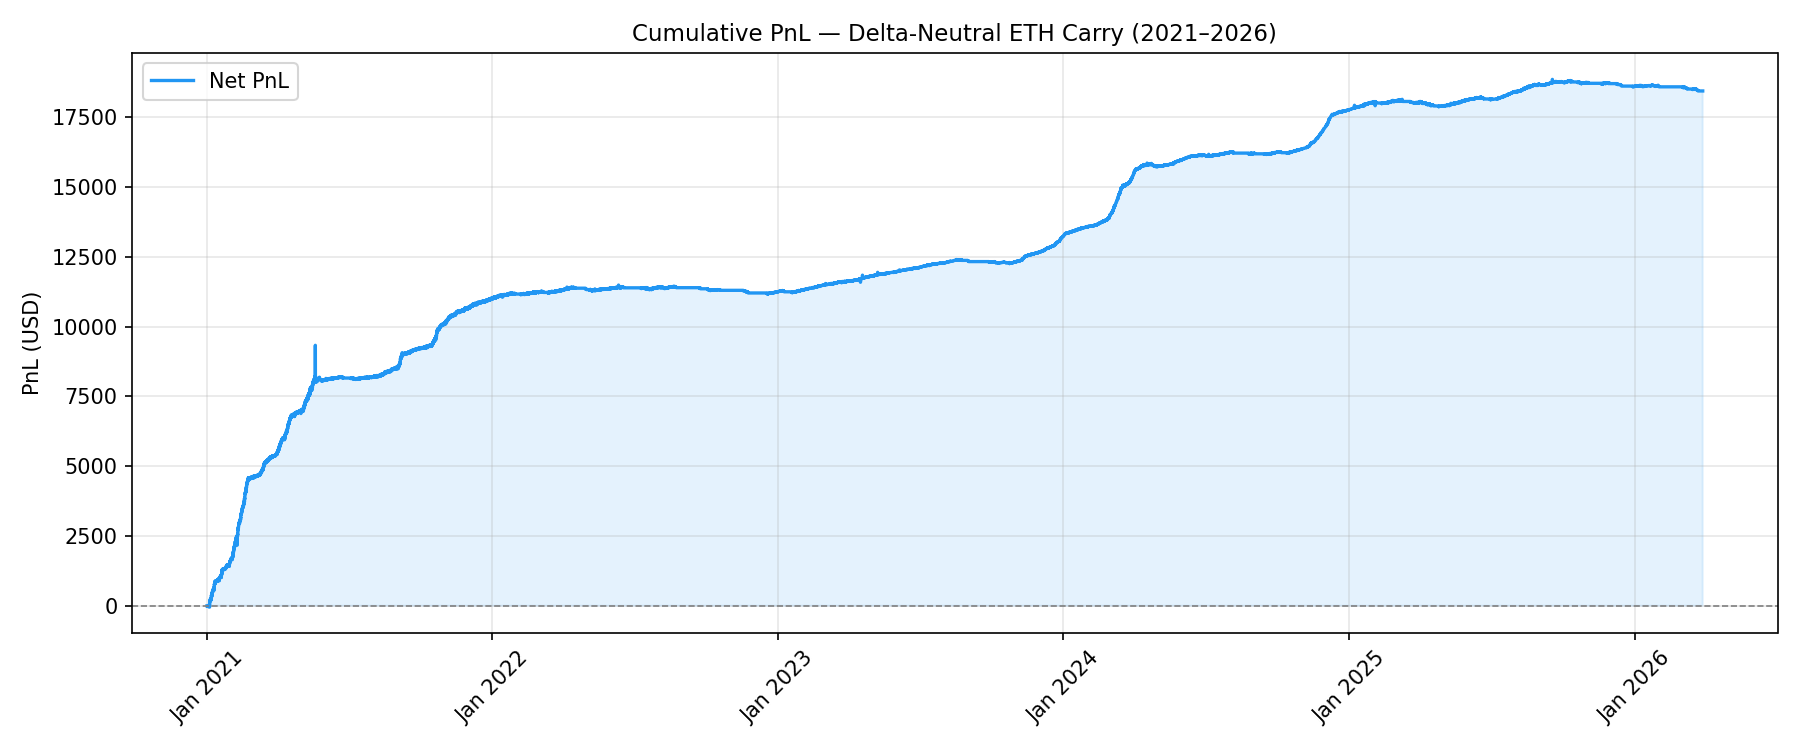
\includegraphics[width=0.9\textwidth]{chart1_cumulative_pnl.png}
    \caption{Cumulative net P\&L (\$) over the full backtest period (Jan 2021 -- Mar 2026).}
    \label{fig:cumulative_pnl}
\end{figure}

\begin{figure}[h!]
    \centering
    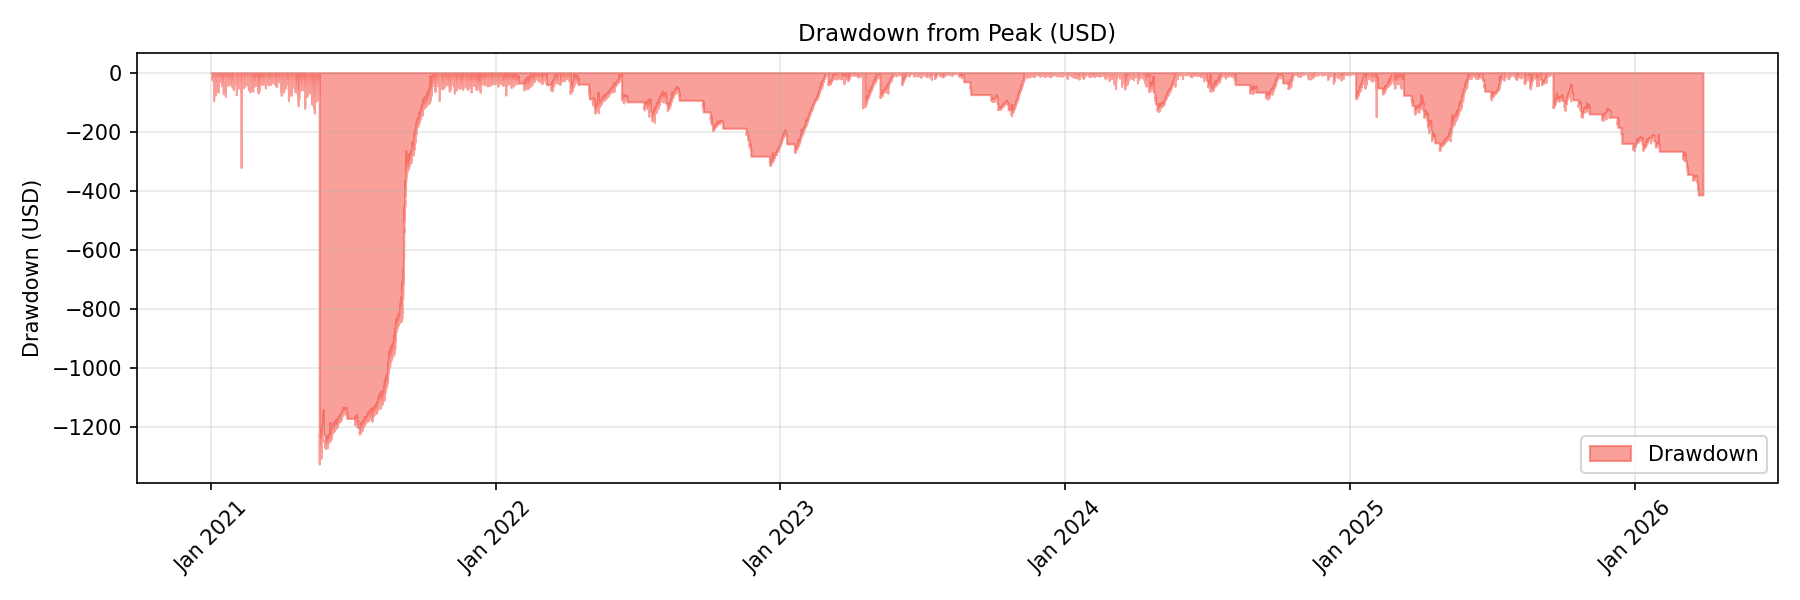
\includegraphics[width=0.9\textwidth]{chart2_drawdown.png}
    \caption{Drawdown from peak equity throughout the backtest period.}
    \label{fig:drawdown}
\end{figure}

\begin{figure}[h!]
    \centering
    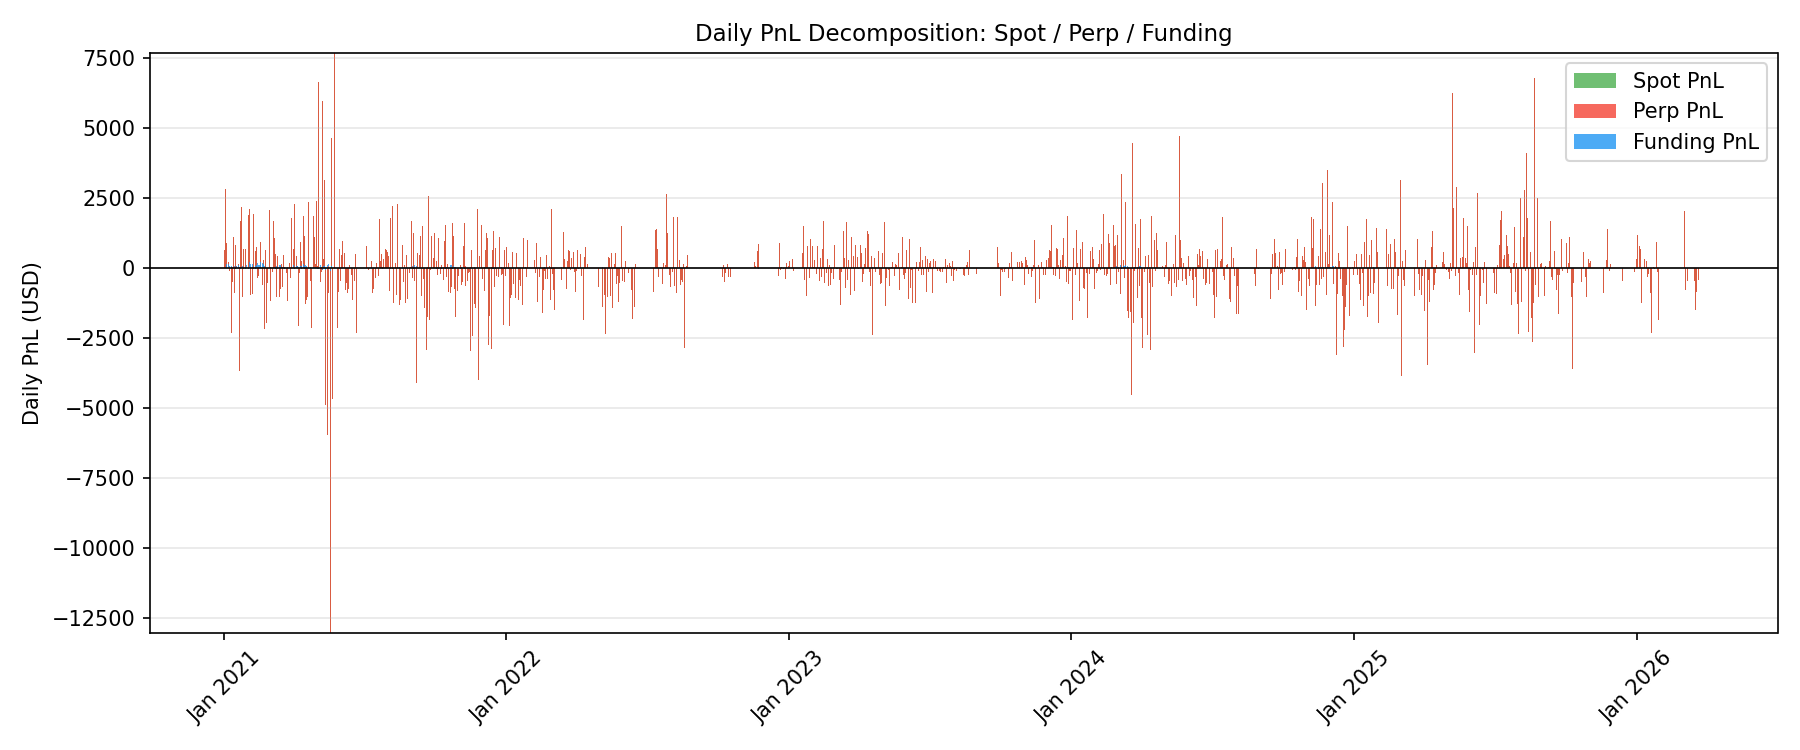
\includegraphics[width=0.9\textwidth]{chart3_pnl_decomposition.png}
    \caption{Daily PnL decomposition: funding carry, spot leg, perp leg.}
    \label{fig:decomposition}
\end{figure}

\textbf{Performance Table --- With Carry Gate (primary result):}

\begin{table}[h!]
\centering
\caption{Performance summary with carry gate active.}
\begin{tabular}{@{}ll@{}}
\toprule
\textbf{Metric} & \textbf{Value} \\
\midrule
Period                       & Jan 2021 -- Mar 2026 ($\approx$1,912 days) \\
Days in position             & $\approx$1,507 / 1,912 (79\%) \\
Days in cash (gate closed)   & $\approx$405 (21\%) --- bear/backwardation periods \\
\textbf{Net PnL}             & \textbf{+\$18,442} \\
Total return                 & +184.4\% \\
Annualised return            & \textbf{+35.2\%} \\
Daily Sharpe                 & \textbf{6.59} (see caveat below) \\
Max drawdown                 & $-$\$1,326 ($-$13\%) \\
\bottomrule
\end{tabular}
\end{table}

\textbf{Sharpe caveat:} The full-period Sharpe of 6.59 is heavily influenced by elevated funding conditions during the 2021 bull market. From 2022 onwards in a flat/bear environment, the Sharpe drops to approximately \textbf{0.4}. Out-of-position days (gate closed) contribute zero variance, mechanically raising the ratio further. Treat the full-period figure as historical context, not a stable forward estimate.

See \texttt{output/tables/backtest\_metrics.csv} for the machine-readable summary.

\subsection{Key Findings}

\textbf{1. The carry gate is the strategy.} The gate exits during bear markets when funding turns negative (backwardation), protecting capital and sitting in USDC. This validates the core design decision in \texttt{StrategyVault.sol}. The strategy was active 79\% of the period, sitting out the worst bear-market stretches.

\textbf{2. Funding is the return driver.} Net price PnL on the two legs is approximately zero --- the spot and perp legs cancel as intended. All net income comes from the funding carry leg collected on the short perpetual position.

\textbf{3. Transaction cost discipline matters.} At daily gate granularity, costs are manageable. Hourly gate granularity would produce hundreds of roundtrips, wiping out returns entirely. This confirms that the on-chain \texttt{openHedge}/\texttt{closeHedge} owner-controlled design (not automated every bar) is the right call.

\textbf{4. Sharpe caveat.} The full-period Sharpe of 6.59 is influenced by two factors: (a) elevated funding conditions during the 2021 bull market that are unlikely to repeat every cycle; (b) out-of-position days (gate closed) contribute zero variance, mechanically raising the ratio. From 2022--2026 alone, the Sharpe is approximately 0.4. The return and drawdown figures are more meaningful for evaluating strategy viability.

\textbf{5. Known methodological limitations (disclosed, not hidden):}
\begin{itemize}
    \item Position is resized at each re-entry but not rebalanced intra-position. Hedge ratio drifts slightly over each holding period.
    \item No slippage, borrow cost, or liquidation mechanics modelled.
    \item Assumes perfect fills at hourly close prices.
\end{itemize}

% ============================================================
\section{Frontend}
% ============================================================

\subsection{Description}

A minimal HTML/JS dashboard (\texttt{frontend/index.html}) connects to deployed Sepolia contracts via MetaMask and ethers.js v6. Features: wallet connect, vault state display including \texttt{netDeltaPnL}, deposit, withdraw, open/close position, oracle price display, carry viability check.

\subsection{Screenshot}

\textit{TODO: add after connecting MetaMask to Sepolia contracts.}

% ============================================================
\section{Gas Analysis and Optimisation}
% ============================================================

\subsection{Gas Report Summary}

Gas figures from \texttt{gas-report.txt} (Solidity 0.8.24, optimizer enabled, 200 runs):

\begin{table}[h!]
\centering
\caption{Detailed gas cost breakdown.}
\begin{tabular}{@{}lrrl@{}}
\toprule
\textbf{Operation} & \textbf{Gas (avg)} & \textbf{\% block limit} & \textbf{Notes} \\
\midrule
\texttt{openHedge()}     & 333,486 & 0.56\% & Oracle + approve + external call \\
\texttt{deposit()}       & 169,892 & 0.28\% & Share mint + USDC transfer \\
\texttt{closeHedge()}    & 109,799 & 0.18\% & closeShort + USDC return \\
\texttt{accrueFunding()} &  57,846 & 0.10\% & Single storage write \\
\texttt{withdraw()}      &  65,841 & 0.11\% & Share burn + USDC transfer \\
\bottomrule
\end{tabular}
\end{table}

All operations use well under 1\% of Ethereum's block gas limit (60M gas).

\subsection{Gas Optimisations Implemented}

\textbf{1. Solidity optimizer enabled (200 runs)}

\begin{lstlisting}[style=javascript, caption={Optimizer configuration in \texttt{hardhat.config.ts}.}]
// hardhat.config.ts
optimizer: { enabled: true, runs: 200 }
\end{lstlisting}

This tells the compiler to optimise for contracts called frequently (200 times). The compiler inlines small functions, eliminates dead code, and reduces bytecode size, lowering deployment and call costs.

\textbf{2. \texttt{immutable} variables for core addresses}

\begin{lstlisting}[style=solidity, caption={\texttt{immutable} state variables in \texttt{StrategyVault}.}]
IERC20       public immutable usdc;
IPerpEngine  public immutable perpEngine;
IPriceOracle public immutable oracle;
\end{lstlisting}

\texttt{immutable} variables are embedded directly into bytecode at deployment. Reading them costs $\approx$3 gas (\texttt{PUSH} opcode) vs 2,100 gas for a cold \texttt{SLOAD} from regular storage --- a $\approx700\times$ reduction per read. \texttt{openHedge()} reads all three, saving $\approx$6,300 gas per call.

\textbf{3. Pure math library (\texttt{ArbitrageMath})}

All financial calculations are in a stateless \texttt{library}. Library calls use \texttt{JUMP} (cheap) not \texttt{CALL} (expensive). No storage reads inside the math functions --- all inputs passed as parameters.

\textbf{4. Early revert pattern (fail fast)}

All \texttt{require} checks execute before any state changes:

\begin{lstlisting}[style=solidity, caption={Early-revert ordering in \texttt{openHedge()}.}]
require(!hedgeIsOpen, "already open");        // cheapest check first
require(notional > 0, "zero notional");
require(carryScore > threshold, "low carry"); // most expensive last
\end{lstlisting}

Failed transactions revert early, refunding unused gas to the caller.

\textbf{5. Tight storage packing}

\begin{lstlisting}[style=solidity, caption={Adjacent bool for storage packing.}]
bool    public hedgeIsOpen;                   // packed with adjacent uint256
int256  public currentDailyFundingRateBps;
uint256 public hedgeOpenTimestamp;
\end{lstlisting}

Booleans declared adjacent to other variables allow the compiler to pack them into the same 32-byte storage slot, reducing \texttt{SSTORE} costs.

\textbf{6. \texttt{view} functions for all reads}

\texttt{getVaultState()}, \texttt{getUserValue()}, \texttt{isCarryViable()}, \texttt{shouldAutoExit()} are all \texttt{view} --- zero gas when called off-chain (frontend, Etherscan). Only costs gas when called from another contract.

\subsection{What Was Not Optimised (and Why)}

\begin{itemize}
    \item \textbf{No assembly / Yul:} All math uses standard Solidity. Assembly would reduce gas further but significantly reduces readability and auditability --- inappropriate for a proof-of-concept.
    \item \textbf{No custom errors:} Solidity custom errors (\texttt{error InsufficientCarry()}) save $\approx$50 gas per revert vs \texttt{require} strings. Not implemented here to keep the code readable for review.
    \item \textbf{No packed structs for UserInfo:} \texttt{UserInfo \{shares, principal\}} uses two separate \texttt{uint256} slots. Packing into \texttt{uint128} each would halve storage cost but introduces precision risk for high-value positions.
\end{itemize}

% ============================================================
\section{Limitations and Risks}
% ============================================================

\subsection{Mock Exchange}
\texttt{MockPerpEngine} does not model order books, slippage, counterparty risk, funding rate caps, or partial fills. Real execution on a CEX (Binance, Bybit) or DEX (dYdX, GMX) would incur additional costs.

\subsection{Funding Rate Risk}
Backwardation periods (negative funding) cause the strategy to lose carry income. Sustained backwardation (as seen in bear markets) can produce extended losses even though the position is delta-neutral on price.

\subsection{Margin / Liquidation Risk}
The short perp uses $5\times$ leverage. A rapid ETH price spike can erode the collateral buffer faster than funding income accrues, triggering the MARGIN auto-exit or, in an extreme scenario, liquidation by the exchange.

\subsection{No Rebalancing}
The 1:1 hedge ratio drifts over time as ETH price moves. This introduces residual delta risk that grows with position duration and price volatility.

\subsection{Oracle Risk}
Chainlink staleness check (3600 seconds) reduces but does not eliminate oracle manipulation risk. Production systems should use TWAP oracles and circuit breakers.

\subsection{What Would Be Needed for Production}

\begin{itemize}
    \item Real exchange connectivity (Binance API, dYdX v4, Hyperliquid)
    \item Automated delta rebalancing (keeper bot)
    \item Dynamic benchmark rate from a real money market
    \item Cross-margin and multi-asset collateral
    \item Governance for risk parameter updates
\end{itemize}

% ============================================================
\section{Conclusion}
% ============================================================

\subsection{Summary}

The backtest suggests that the delta-neutral ETH carry strategy is mechanically valid and economically plausible over the sampled period, with returns primarily driven by the funding carry leg. The on-chain proof-of-concept correctly implements the mechanism --- including the carry gate, delta-neutral PnL accounting, and four auto-exit conditions. The backtest covers $\approx$1,912 days (Jan 2021 -- Mar 2026) using real Bybit settlement funding rates, spanning a full bull/bear market cycle. Results should be interpreted as historical validation of the strategy design, with the caveat that 2021's elevated funding environment is not representative of typical conditions.

\subsection{What We Learned}

\begin{itemize}
    \item \textbf{Delta-neutrality holds in the model.} Holding equal spot and perp legs cancels price risk. On-chain verification (\texttt{netDeltaPnL} $\approx 0$) confirms the accounting is correct. The stress test (funding $= 0 \Rightarrow$ PnL $\approx 0$) gives the clearest evidence: the net gain is attributable to the funding leg, not to incidental price drift.
    \item \textbf{Funding is the return driver.} The strategy's PnL is explained by real Bybit settlement funding rates. The 2021 bull market drove the majority of profits; the carry gate correctly kept the strategy in cash during 2022's bear market.
    \item \textbf{Carry is not constant and can reverse.} Funding rates are highly variable. Backwardation periods --- common in bear markets --- produce losses even with a correct hedge. The carry gate is the primary defence against this.
    \item \textbf{On-chain precision required care.} Solidity's integer arithmetic with 6-decimal USDC and 18-decimal prices requires careful formula design to avoid precision loss --- and the on-chain tests confirm it is handled correctly.
\end{itemize}

\subsection{Extensions for Future Work}

\begin{itemize}
    \item Implement dynamic delta rebalancing (rebalance when hedge ratio drifts beyond a threshold)
    \item Add a real Aave lending integration for the spot leg to earn additional yield on idle capital
    \item Build a keeper bot for automated \texttt{autoClose()} execution
    \item Extend backtest to include funding rate forecasting for entry/exit timing
\end{itemize}

% ============================================================
\appendix
\section{Formula Reference}
% ============================================================

See \texttt{docs/formulas.md} for the canonical formula reference. Key formulas are reproduced in Section~4 of this report.

% ============================================================
\section{Source Code}
% ============================================================

See \texttt{contracts/} directory. All contracts are verified on Etherscan (links in Section~7.1).

% ============================================================
\section{Backtest Data}
% ============================================================

See \texttt{output/tables/} after running \texttt{python backtest/run\_backtest.py}.

% ============================================================
\section{Demo \& Execution Evidence}
% ============================================================

\subsection*{Deployed Contracts (Sepolia)}

\begin{itemize}
    \item \textbf{MockUSDC} --- \href{https://sepolia.etherscan.io/address/0x84EAb608016e21E4618c63B01F7b3b043F4f457e}{\texttt{0x84EAb608016e21E4618c63B01F7b3b043F4f457e}}
    \item \textbf{ArbitrageToken (CARB)} --- \href{https://sepolia.etherscan.io/address/0xd2E7bA891e0Ecd142695d04e8Ed79e0C4947922F}{\texttt{0xd2E7bA891e0Ecd142695d04e8Ed79e0C4947922F}}
    \item \textbf{ChainlinkPriceOracle} --- \href{https://sepolia.etherscan.io/address/0x27768a80Fb849F6c1bB941C8de62F417Cd968e35}{\texttt{0x27768a80Fb849F6c1bB941C8de62F417Cd968e35}}
    \item \textbf{MockPerpEngine} --- \href{https://sepolia.etherscan.io/address/0x478832D03495390E47aFD238A9bA11414096A452}{\texttt{0x478832D03495390E47aFD238A9bA11414096A452}}
    \item \textbf{StrategyVault} --- \href{https://sepolia.etherscan.io/address/0x036EA2E331994a04d853B54Ad19D05524eC5b399}{\texttt{0x036EA2E331994a04d853B54Ad19D05524eC5b399}}
\end{itemize}

\subsection*{Frontend Screenshot}

\begin{center}
\textit{[Screenshot placeholder --- wallet connected, vault state visible, MetaMask on Sepolia]}
\end{center}

\subsection*{Example Contract Interaction}

\begin{center}
\textit{[Etherscan transaction screenshot placeholder --- \texttt{openHedge()} or \texttt{closeHedge()} call on StrategyVault]}
\end{center}

% ============================================================
\section{References}
% ============================================================

\textbf{Data}
\begin{itemize}
    \item Bybit ETHUSDT historical data --- spot price, perpetual close, and 8h settlement funding rate (\texttt{data/raw/bybit\_eth\_usdt\_1h.csv})
\end{itemize}

\textbf{Technical documentation}
\begin{itemize}
    \item Chainlink Price Feeds --- \url{https://docs.chain.link/data-feeds}
    \item OpenZeppelin Contracts v5 --- \url{https://docs.openzeppelin.com/contracts/5.x/}
    \item Hardhat --- \url{https://hardhat.org/docs}
\end{itemize}

\textbf{Conceptual background}
\begin{itemize}
    \item Bybit perpetual futures and funding rate mechanism --- \url{https://www.bybit.com/en/help-center/article/funding-rate-mechanism}
    \item Perpetual Protocol documentation --- funding rate overview
\end{itemize}

% ============================================================
\end{document}
% ============================================================
